

\usepackage{verbatim, multicol, tabularx,hyperref, tikz, enumitem}
\usepackage{amsmath,amsthm, amssymb, stmaryrd, latexsym, bm, listings, qtree}
\usepackage[margin=1in]{geometry}

\lstset{
  extendedchars=\true,
  inputencoding=utf8,
  literate=
  {é}{{\'{e}}}1
  {è}{{\`{e}}}1
  {ê}{{\^{e}}}1
  {ë}{{\¨{e}}}1
  {û}{{\^{u}}}1
  {ù}{{\`{u}}}1
  {â}{{\^{a}}}1
  {à}{{\`{a}}}1
  {î}{{\^{i}}}1
  {ô}{{\^{o}}}1
  {ç}{{\c{c}}}1
  {Ç}{{\c{C}}}1
  {É}{{\'{E}}}1
  {Ê}{{\^{E}}}1
  {À}{{\`{A}}}1
  {Â}{{\^{A}}}1
  {Î}{{\^{I}}}1
  {Ö}{{\"O}}1
  {Ä}{{\"A}}1
  {Ü}{{\"U}}1
  {ö}{{\"o}}1
  {ä}{{\"a}}1
  {ü}{{\"u}}1
  {ß}{{\ss}}1
  ,
  aboveskip=1mm,
  belowskip=1mm,
  showstringspaces=false,
  columns=flexible,
  basicstyle={\scriptsize\ttfamily},
  numbers=left,
  frame=single,
  framextopmargin=0pt,
  framexbottommargin=0pt,
  breaklines=true,
  breakatwhitespace=true,
  keywordstyle=\color{blue},
  identifierstyle=\color{violet},
  stringstyle=\color{teal},
  commentstyle=\color{darkgray}
}

\hypersetup{colorlinks=true,urlcolor=blue}

\headheight = 0.05 in
\headsep = 0.05 in
\parskip = 0.05in
\parindent = 0.0in
\floatsep = 0.05in

\DeclareMathOperator*{\argmin}{arg\!min}
\DeclareMathOperator*{\argmax}{arg\!max}

\title{MDPs Study Guide (AIMA 17)}
\author{Artificial Intelligence}
\date{}

\begin{document}
\maketitle

\setcounter{section}{0} % So that next \section is 1
\section{Markov Decision Processes}

\begin{questions}

\question What are the components of a Markov Decision Process?

\begin{solution}[3in]
A Markov decision process (MDP) is a 4-tuple $\left( S, A, Pr(s' \mid s, a), R(s) \right)$, where

\begin{itemize}
\item $S$ is a set of states,
\item $A$, or $Action(s)$ is a set of actions, and
\item $Pr(s' \mid s, a)$ is a transition function giving the probability that executing action $a$ in state $s$ will result in $s'$.  Many authors use $T(s, a, s')$
\item  $R(s, a, s')$ is the reward the world provides to an agent for arriving in state $s'$ after executing action $a$ in state $s$, bounded by $\pm R_{max}$.  Many authors use $R(s')$, which is easier to think about -- the reward for arriving in state $s'$ regardless of the $s, a$ pair in the previous time step.
\end{itemize}

Some definitions of MDPs include an initialization function, $I(s)$, which specifies the probability the the agent will start in some state $s \in S$, others specify a particular state $s_0$ from $S$ as the start state.
\end{solution}



\question  What is the role of $\gamma$ in the calculation of infinite horizon returns, $G_t = \sum_{k = 0}^\infty \gamma^k r_{t+k+1}$?

\begin{solution}[.5in]
To discount the value of future rewards.
\end{solution}

\end{questions}

\newpage

\section{Policies}

\begin{questions}

\question In the context of Markov Decision Processes, what is a policy?

\begin{solution}[1in]
The solution to an MDP is a policy, which is a function that returns a recommended action for every state, denoted $\pi(s)$.
\end{solution}

\question In the context of Markov Decision Processes, what is a stochastic policy?

\begin{solution}[1in]
A stochastic policy is a probability distribution over actions conditioned on the state, $\pi(a \mid s)$.
\end{solution}


\question How many optimal policies are there in an MDP?

\begin{solution}[.5in]
At least one
\end{solution}

\question Given the following optimal state values:

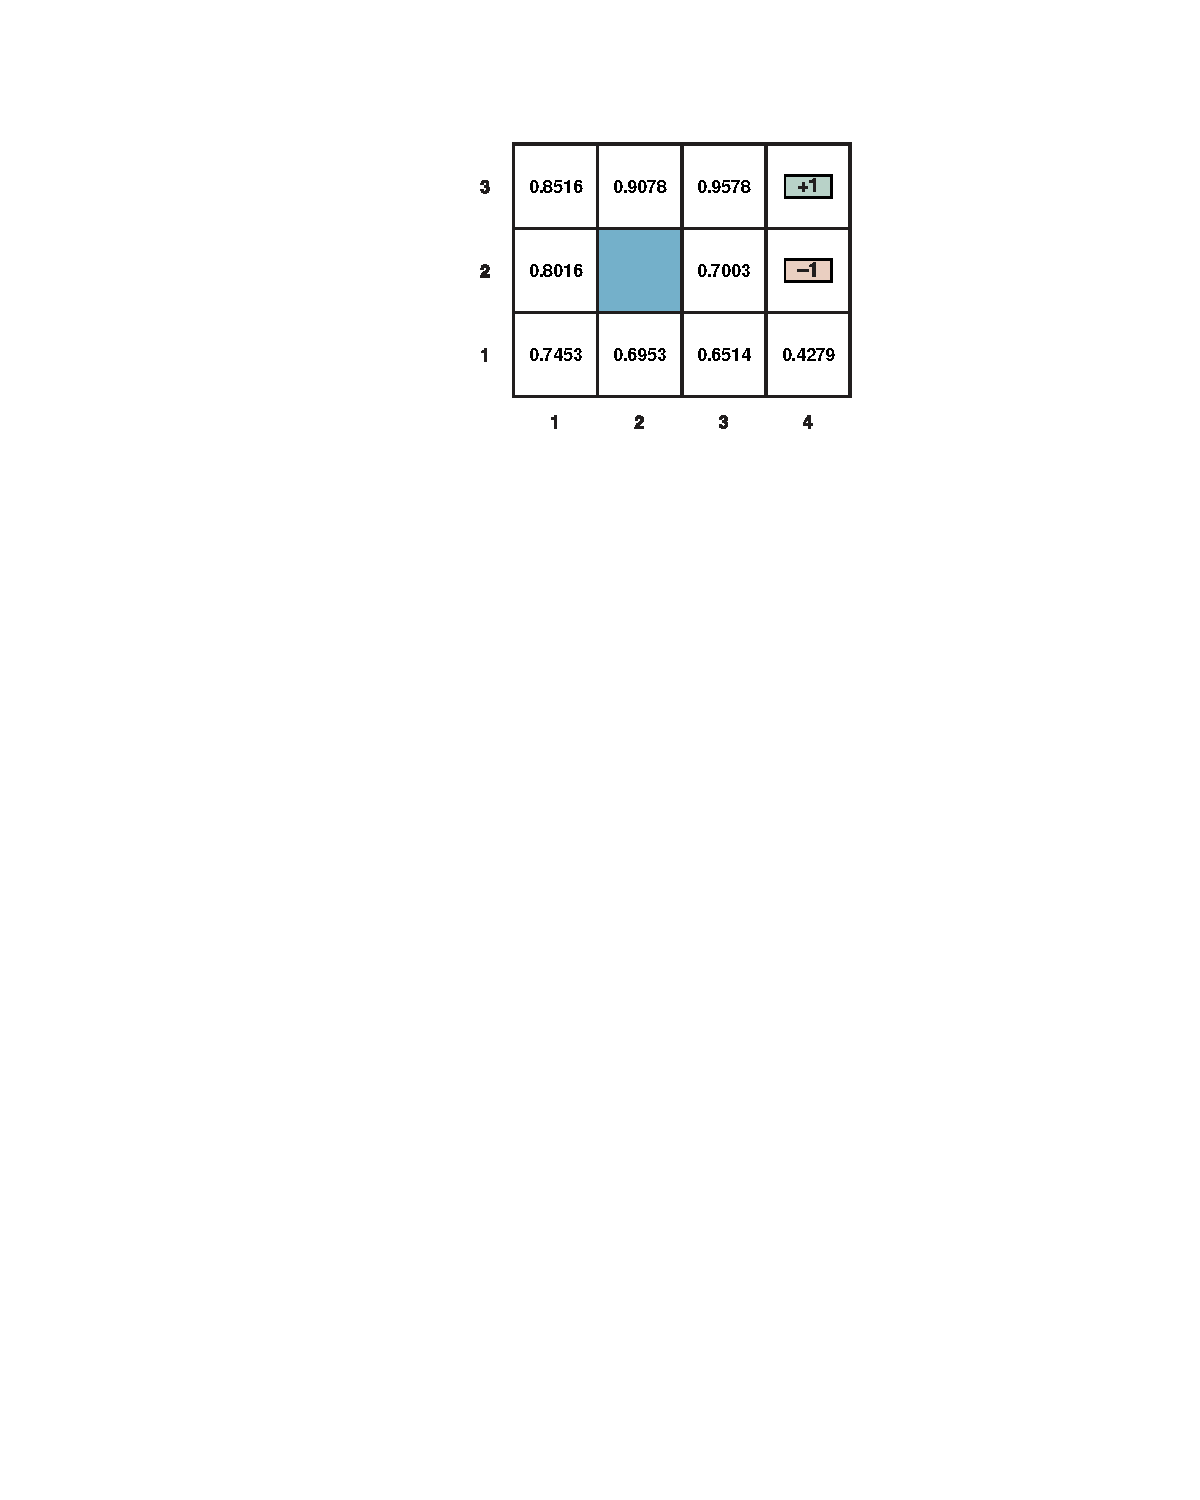
\includegraphics[height=1.5in]{aima-fig-17_03-state-values.pdf}

What is the deterministic optimal policy, $\pi(s)$?

\ifprintanswers
\begin{tabular}{|p{1.25in}|p{1.25in}|p{1.25in}|p{1.25in}|}\hline
$\pi((1, 3)) = Right$ & $\pi((2, 3)) = Right$ & $\pi((3, 3)) = Right$ & $\pi((4, 3)) = Noop$ \\\hline
$\pi((1, 2)) = Up$    &                       & $\pi((3, 2)) = Up$    & $\pi((4, 2)) = Noop$ \\\hline
$\pi((1, 1)) = Up$    & $\pi((2, 1)) = Left$  & $\pi((3, 1)) = Up$    & $\pi((4, 1)) = Left$ \\\hline
\end{tabular}
\else
\vspace{2in}
\fi

\end{questions}

\end{document}
